\item Prism 1 with bar 2 of mass \( m \) placed on it gets a horizontal acceleration \( w \) directed to the left (Fig. 1.23). At what maximum value of this acceleration will the bar be still stationary relative to the prism, if the coefficient of friction between them \( k < \cot \alpha \)?
    \begin{center}
        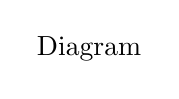
\begin{tikzpicture}
            \node at (0, 0) {Diagram};
        \end{tikzpicture}
    \end{center}
\begin{solution}
    \begin{center}
        \begin{tikzpicture}
            \pic at (0, 0) {frame=3cm};
        \end{tikzpicture}
    \end{center}
    
    \begin{align*}
        \intertext{On the basis of the initial argument of the solution of problem 1.79, the tendency of bar 2 with respect to 1 will be to move up along the plane.}
        \intertext{Let us fix $x-y$ coordinate system in the frame of ground as shown in the figure.}
        \intertext{From second law of motion in projection form along $y$- and $x$-axes}
        mg \cos \alpha - N &= mw \sin \alpha\\
        \intertext{or}
        N &= m \left(g \cos \alpha - w \sin \alpha \right) \tag{1}
        \intertext{}
        mg \sin \alpha + fr &= mw \cos \alpha\\
        \intertext{or}
        fr &= m \left(w \cos \alpha - g \sin \alpha \right) \tag{2}
        \intertext{but}
        fr &\leq kN\\
        \intertext{So from Eqs. (1) and (2),}
        \left(w \cos \alpha - g \sin \alpha \right) &\leq k \left(g \cos \alpha + w \sin \alpha \right)\\
        \intertext{or}
        w \left(\cos \alpha - k \sin \alpha \right) &\leq g \left(k \cos \alpha + \sin \alpha \right)\\
        \intertext{or}
        w &\leq g \frac{\left(k \cos \alpha + \sin \alpha \right)}{\cos \alpha - k \sin \alpha}\\
        \intertext{So, the sought maximum acceleration of the wedge is}
        w_{\text{max}} &= g \frac{\left(k \cos \alpha + \sin \alpha \right)}{\cos \alpha - k \sin \alpha} = g \frac{\left(k \cot \alpha + 1 \right)}{\cot \alpha - k} \quad \text{where } \cot \alpha > k
    \end{align*}
\end{solution}
